\documentclass[12pt,letterpaper]{article}
\usepackage[utf8]{inputenc}
\usepackage{times}
\usepackage{authblk}
\usepackage{graphicx}
\usepackage{placeins}
\usepackage{pdfpages}

\title{StudyUp - Software Design Specification and User Interface}

\author[1]{Yukon Vinecki}
\author[2]{Chandler Petersen}
\author[3]{Calvin Todorovich}
\author[4]{Moyez Ikhlas}
\affil[1]{vineckiy, EECS - Oregon State University}
\affil[2]{petercha, EECS - Oregon State University}
\affil[3]{todorovc, EECS - Oregon State University}
\affil[4]{ikhlasm, EECS - Oregon State University}

% Don't indent new paragraphs, avoids unnecessary new lines
\usepackage[parfill]{parskip}
\begin{document}

\pagenumbering{roman}
\maketitle
\clearpage
\tableofcontents
\clearpage
\pagenumbering{arabic}

\section{User Interface Prototypes}
\subsection{UI Prototype Descriptions}
Home Page: From the Home Page UI, the user can view all the study groups to which they currently belong. They then have the option to click on any of these groups, which will take them to the View Group page. In the event that the user is not currently in a group, the default Home Page is the Create Group page. Additionally, the user has the option to use the above navigation-bar to create a group, join a group, or log out of the system.

Create Group: From the Create Group UI, the user has the option to select one of their classes to create a study group for. Doing this brings you to the Create Group Form.

Create Group Form: The purpose of this form is so the user can fill out the relevant information for the study group they are creating. Once the user has filled out the fields in the form, they can hit the "confirm" button, which then brings them to the View page.

View: In the View UI, the user may view the information that was filled out in the group form. If the user is the group administrator, they will have the option to edit the form. If they did not create the group, then they have the options to join or leave the group. The View UI can be reached from Create Group Form UI, the Join UI, and the Home Page UI.

Join Group: The Join UI gives the user the option to select an active study group to join. The groups are sorted by class and by popularity. Clicking on an active group in this UI brings the user to the View page. From here, they can join the selected group. 
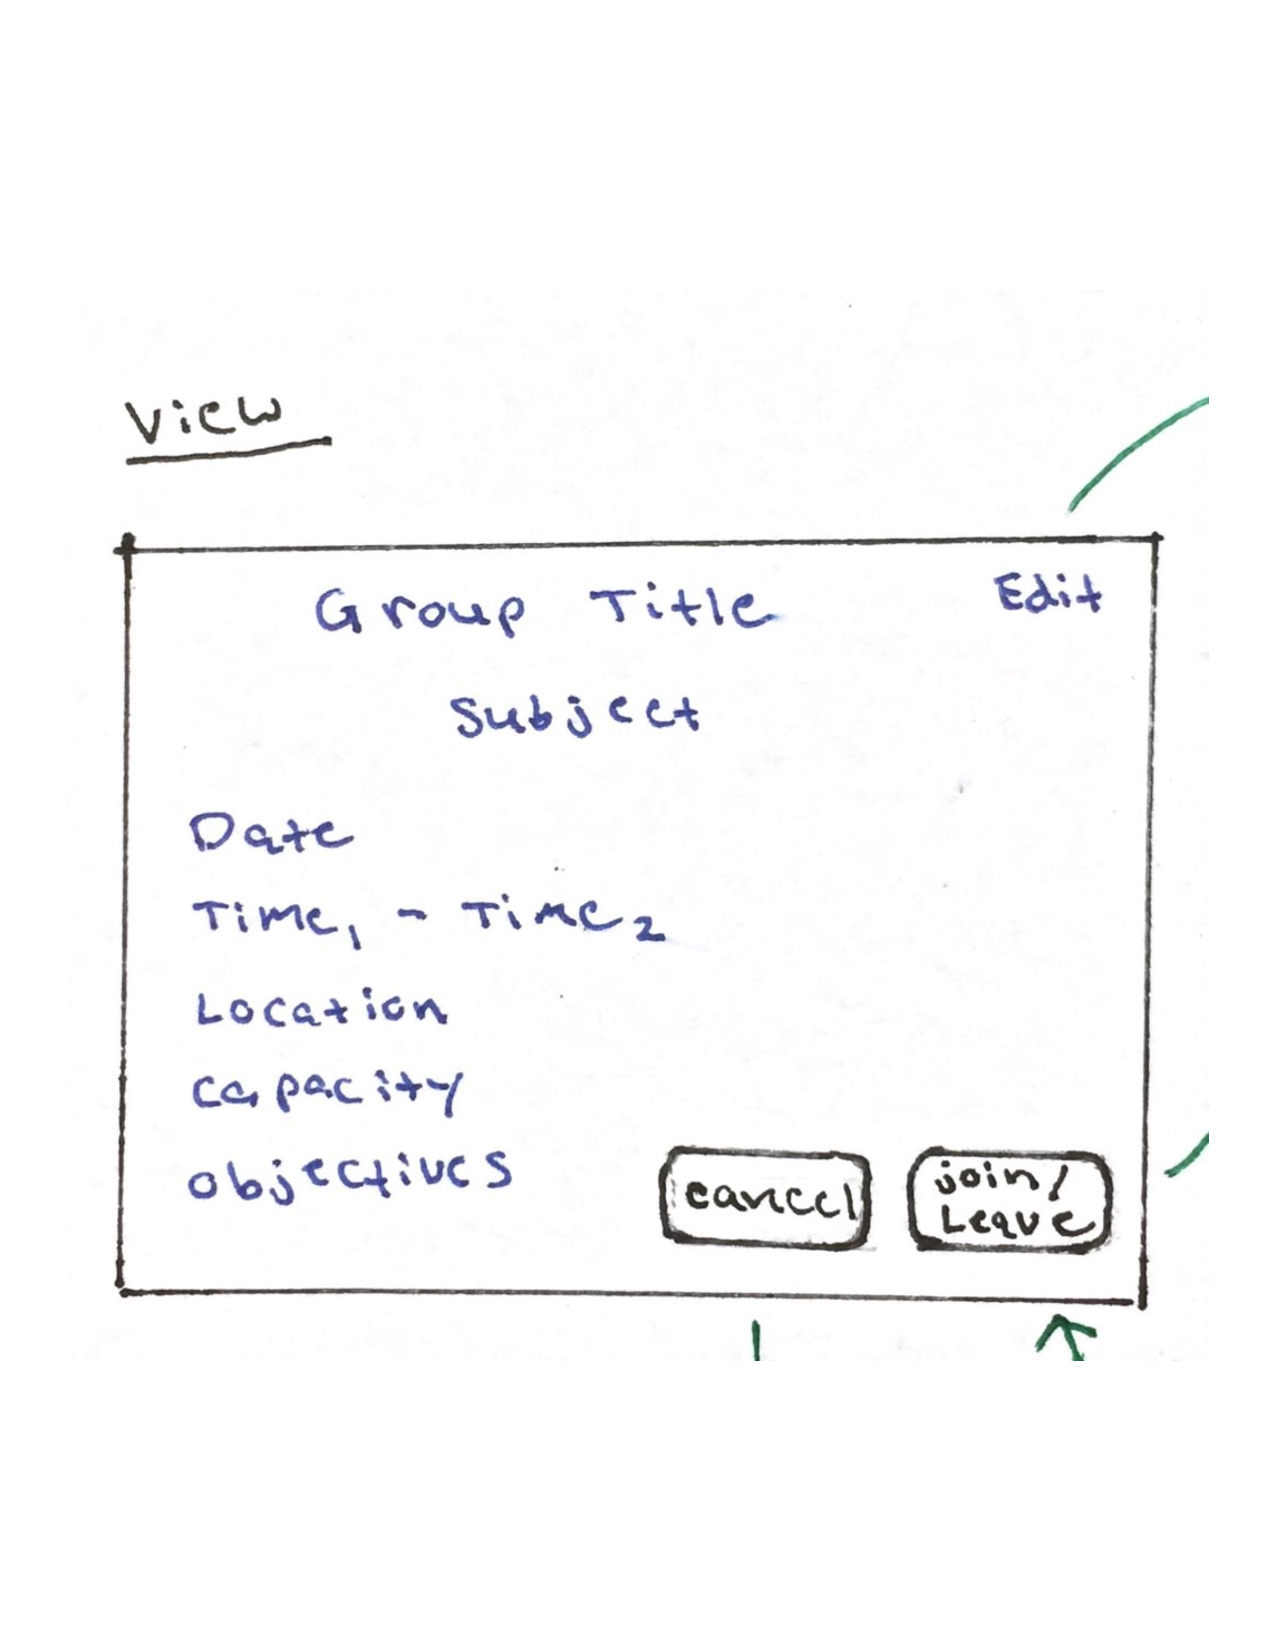
\includepdf[pages={1-5}]{StudyUp_UI_Mocks_2.pdf}
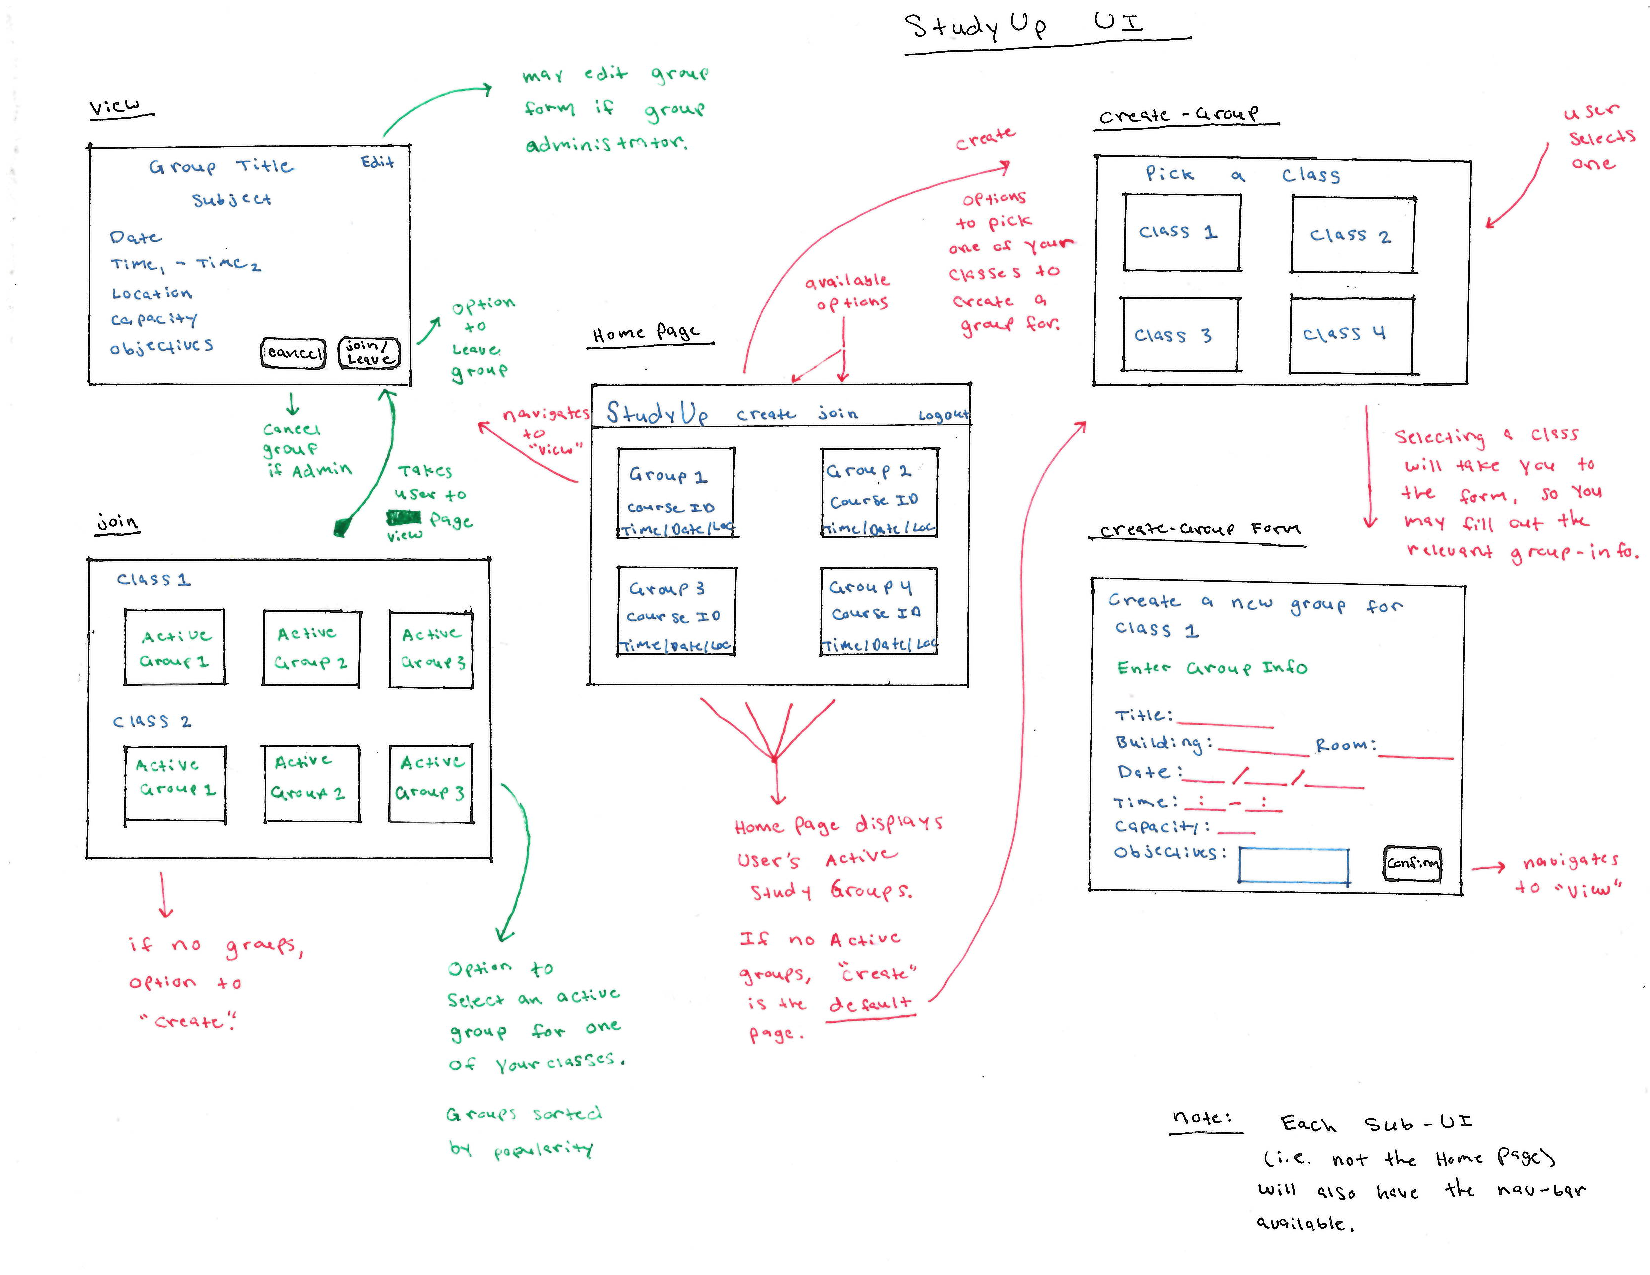
\includepdf[pages={1}]{StudyUp_UI_Mocks.pdf}



\clearpage
\section{Class Diagram}
\begin{figure}[!htb]
  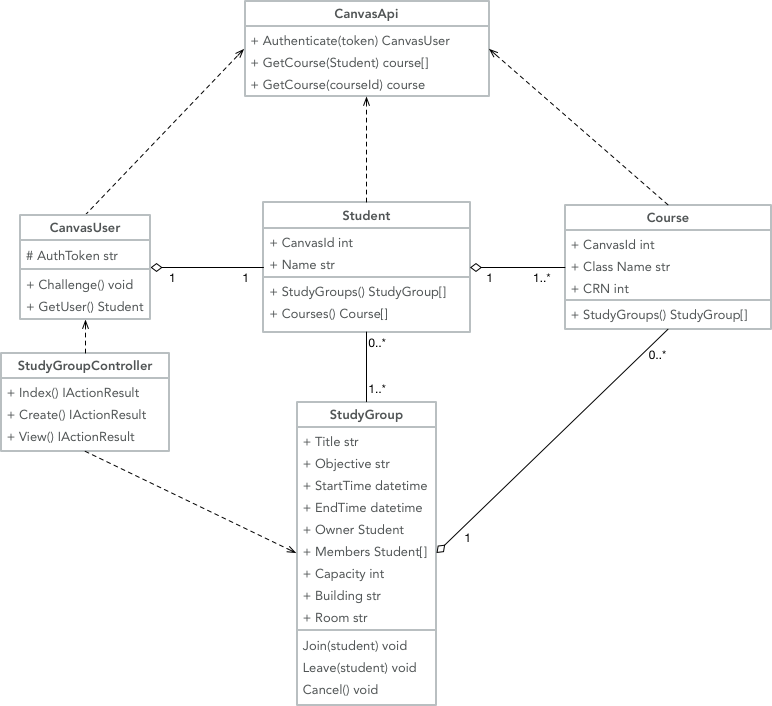
\includegraphics[width=\linewidth]{StudyUp_Class_Diagram.png}
  \caption{Class Diagram}
  \label{class_diagram}
\end{figure}

\clearpage
\section{Sequence Diagrams}
\subsection{Create Study Group}
\begin{figure}[!htb]
  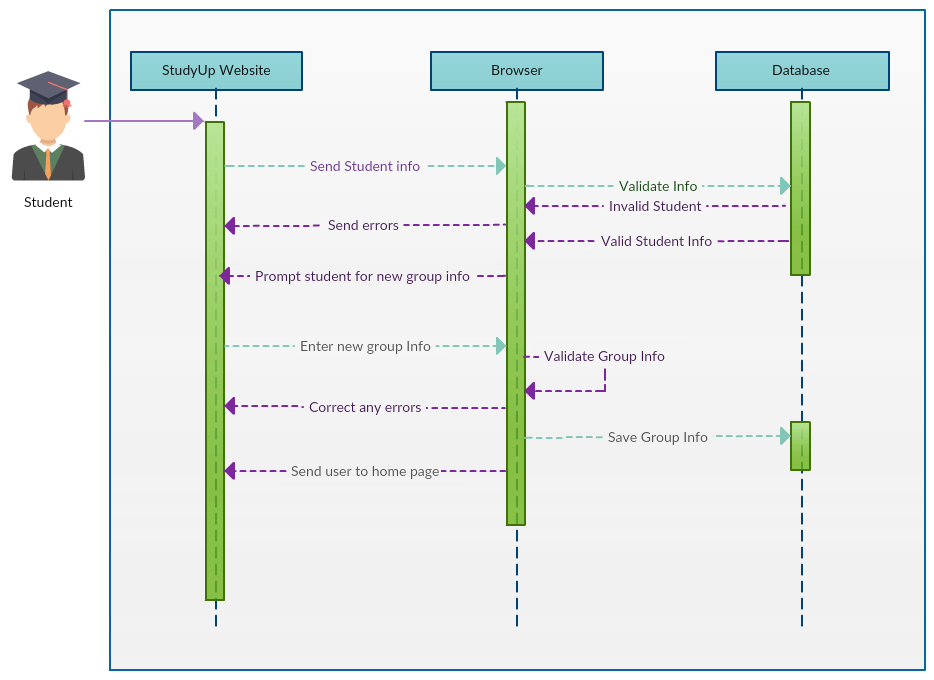
\includegraphics[width=\linewidth]{Create_Study_Group.png}
  \caption{Create sequence diagram}
  \label{create_sequence}
\end{figure}

\clearpage
\subsection{Join Study Group}
\begin{figure}[!htb]
  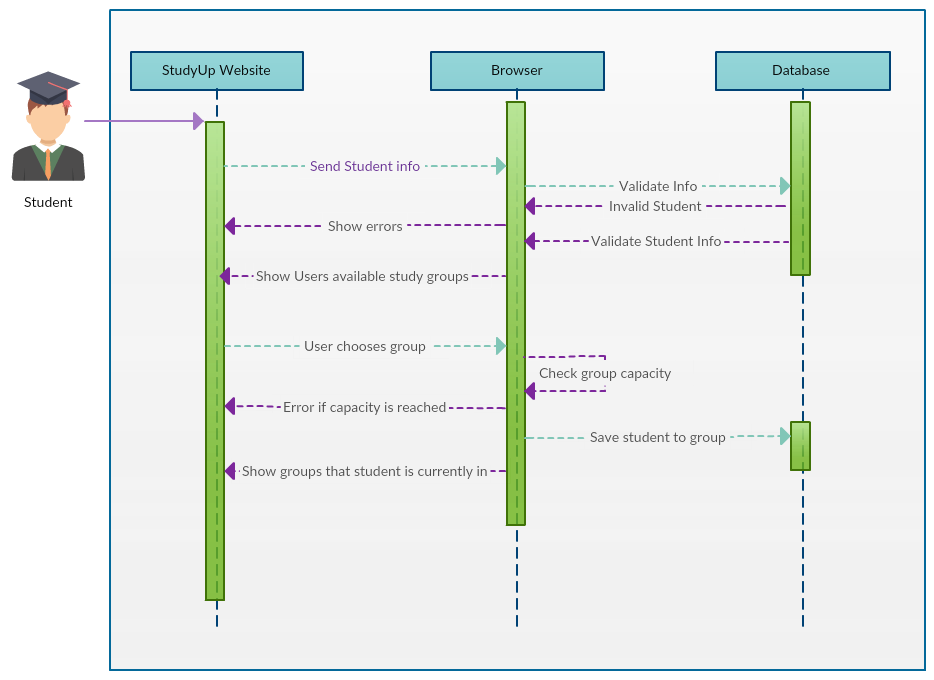
\includegraphics[width=\linewidth]{Join_Study_Group.png}
  \caption{Join sequence diagram}
  \label{join_sequence}
\end{figure}

\clearpage
\subsection{View Study Groups}
\begin{figure}[!htb]
  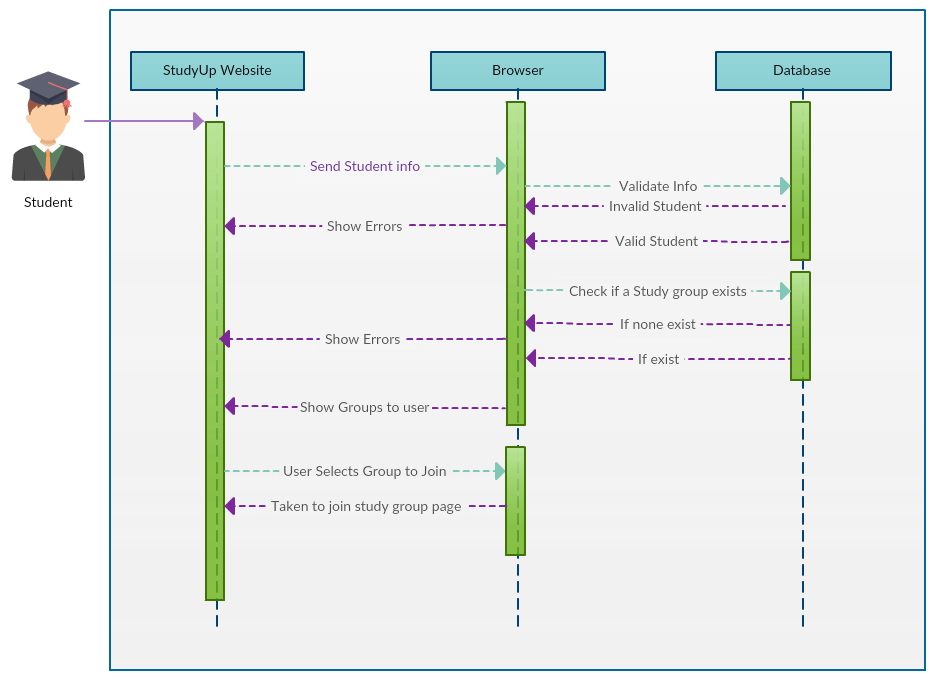
\includegraphics[width=\linewidth]{View_Study_Groups.png}
  \caption{View sequence diagram}
  \label{view_sequence}
\end{figure}

\clearpage
\section{Meeting Report}
We had our weekly Friday meeting again this week with the goal of finalizing prototypes. All members of the team, including the customer, were able to meet and finalize their designs. With prototypes now finalized work can begin on creating the web pages and implementing functionality. There was also discussion on having another time during the week for a work session. 

Each group member worked on designing the prototype of their portion of the UI during the meeting session. Yukon got all group members set up with the framework we are using for development. 

Our goals for next week are for each member to begin creating their assigned portion of the UI/application. Chandler will work on the View UI, Yukon will work on setting up the production server, Calvin will work on the Create Study Group UI, and Moyez will work on the Find Study Group UI. By next week, our goal is to have the HTML and CSS for each UI complete. 
\end{document}